\documentclass[fleqn]{article}

\usepackage{mydefs}
\usepackage{notes}
\usepackage{url}
\usepackage{amsmath}
\usepackage{graphicx}
\graphicspath{ {images/} }
\usepackage{verbatim}
\usepackage{subfig}
\usepackage[rightcaption]{sidecap}


\begin{document}
\lecture{Computer Vision}{Mini Project 03}
{Name:Abhay Doke {UID:29552668}}



\textbf{\huge 1.Scale-space blobs detection}


Images Used for hybrid images:
\vspace{10 mm}


\begin{center}
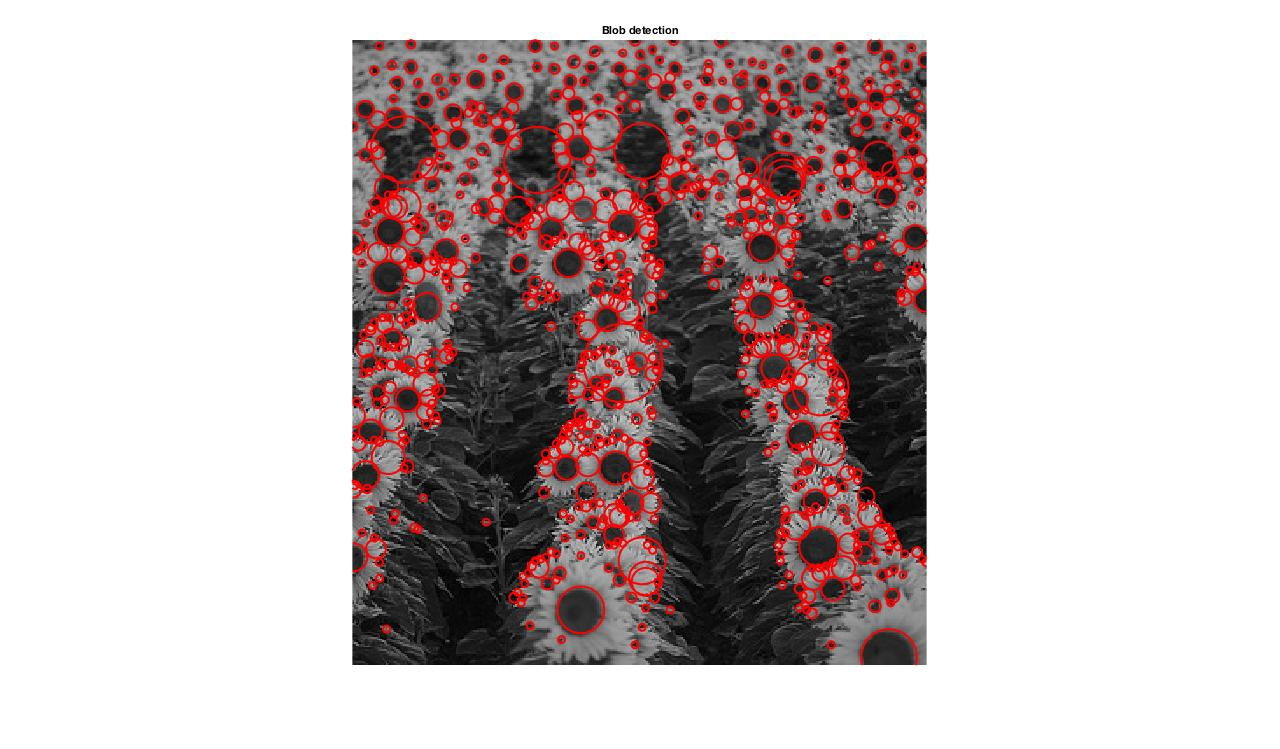
\includegraphics[width=1.2\textwidth]{sunflowers.jpg}

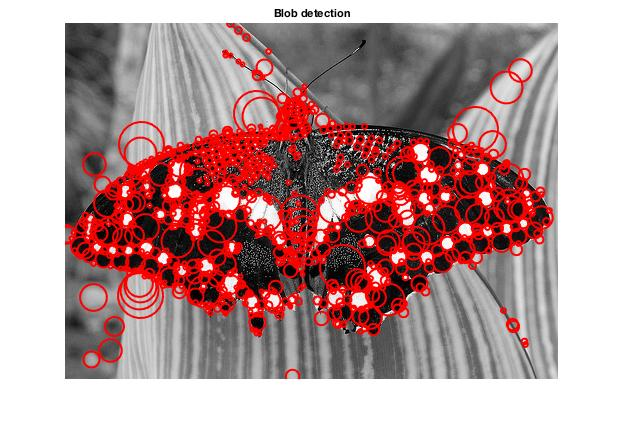
\includegraphics[width=1\textwidth]{butterfly.jpg}
\newline
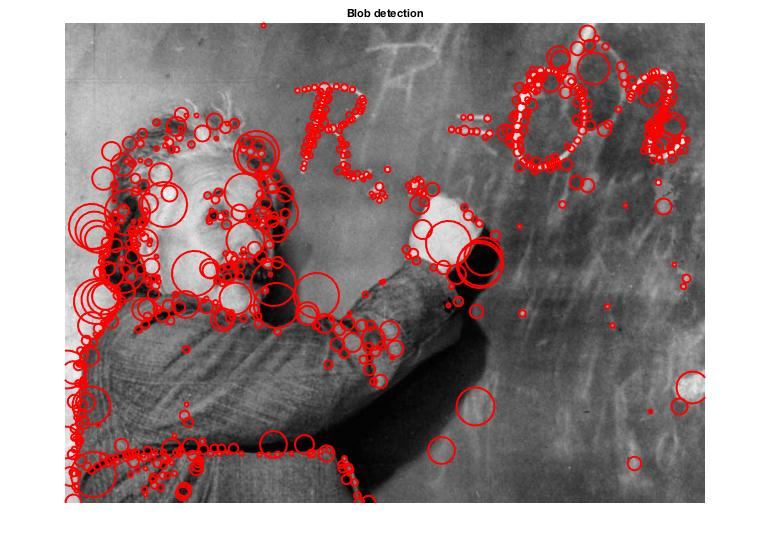
\includegraphics[width=1.2\textwidth]{einstein.jpg}
\newline
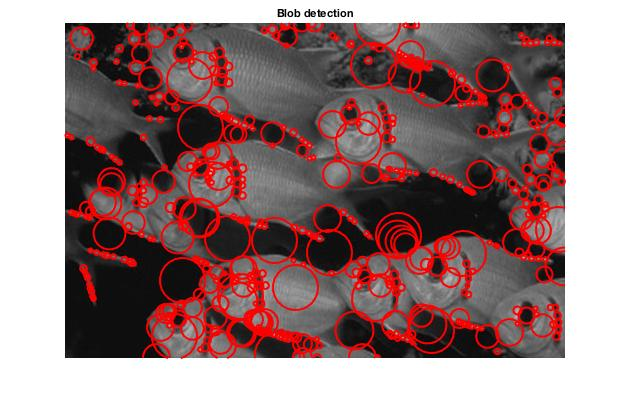
\includegraphics[width=1.2\textwidth]{fishes.jpg}
\end{center}

\newpage

\vspace{10 mm}
Code for \textbf{detectBlobs.m}

\verbatiminput{detectBlobs.m}

\newpage

\textbf{\huge 2. Image Stitching}

\vspace{10 mm}

Results for Hill.jpg
\begin{center}
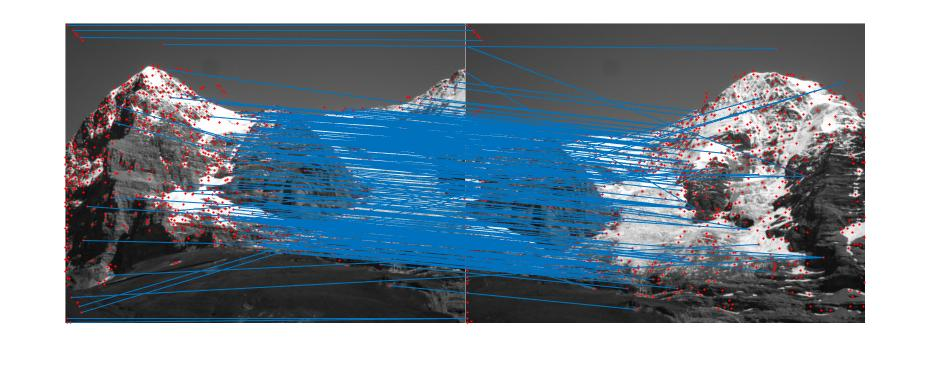
\includegraphics[width=1.2\textwidth]{hill1.jpg}

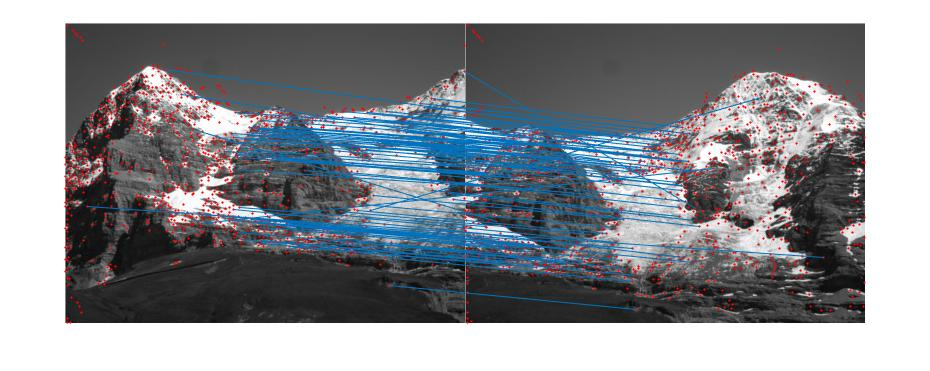
\includegraphics[width=1.2\textwidth]{hill2.jpg}
\newline
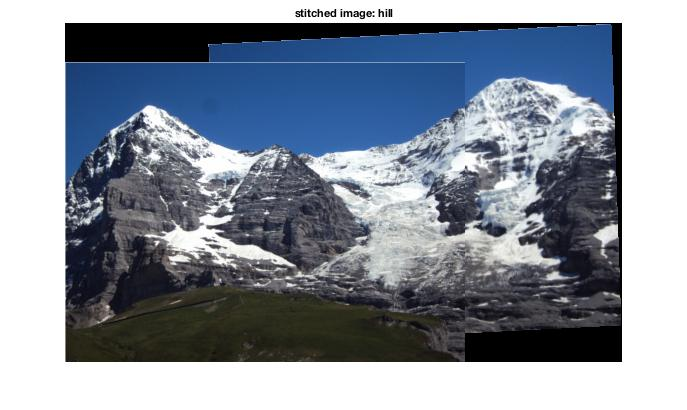
\includegraphics[width=1.2\textwidth]{hill3.jpg}

Affine Transformation Matrix:
\vspace{10 mm}

Hill.jpg

1.0102   ,   0.0333   ,   142.8521;

-0.0513  ,   1.0090   ,  -18.2562;

\end{center}

\newpage

Results for Field.jpg
\begin{center}
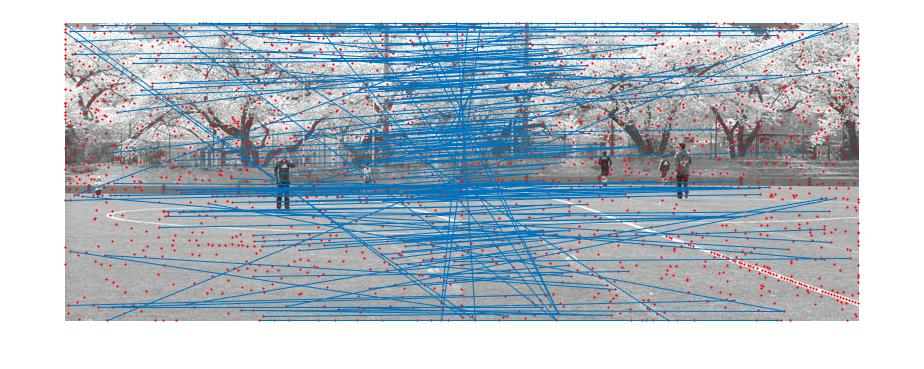
\includegraphics[width=1.2\textwidth]{field1.jpg}

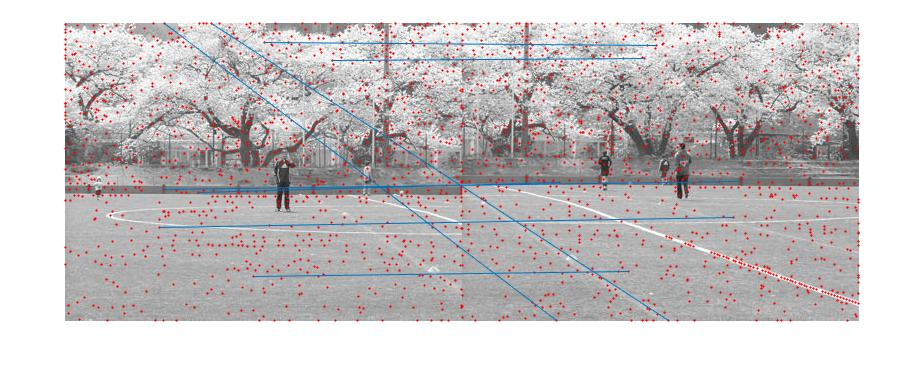
\includegraphics[width=1.2\textwidth]{field2.jpg}
\newline
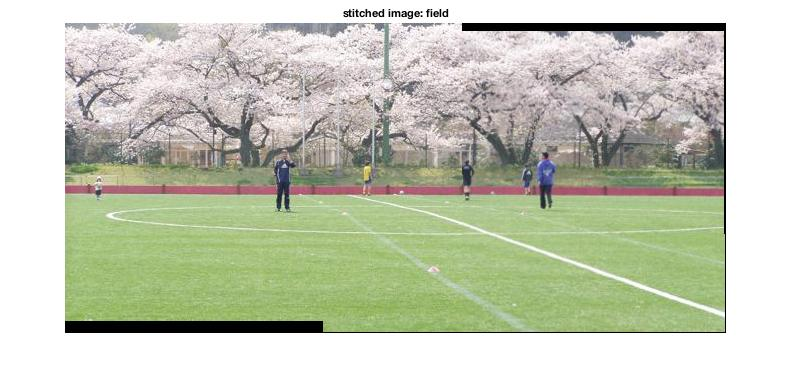
\includegraphics[width=1.2\textwidth]{field3.jpg}

Affine Transformation Matrix:
\vspace{10 mm}

Field.jpg

0.9996   ,   0.0112   ,    256.6738;

-0.0004  ,   1.0112   ,      8.6738;

\end{center}

\newpage

Results for Ledge.jpg
\begin{center}
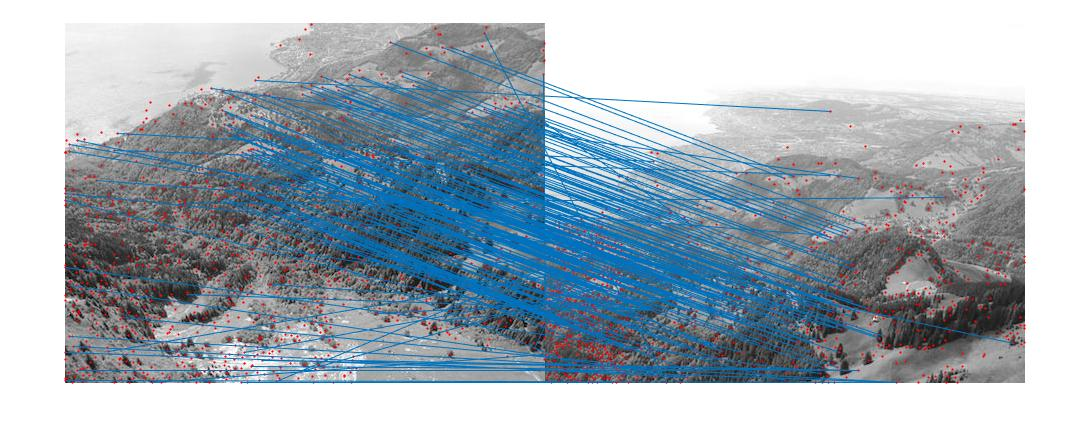
\includegraphics[width=1.2\textwidth]{ledge1.jpg}

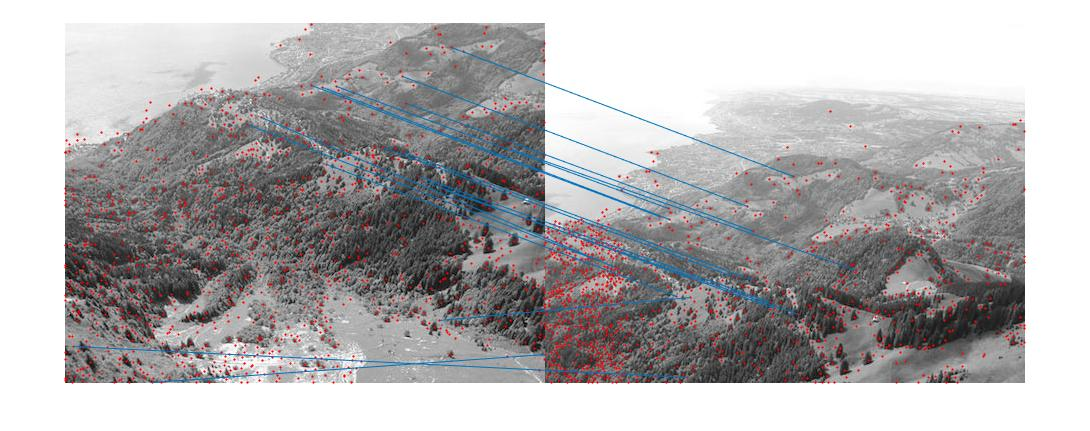
\includegraphics[width=1.2\textwidth]{ledge2.jpg}
\newline
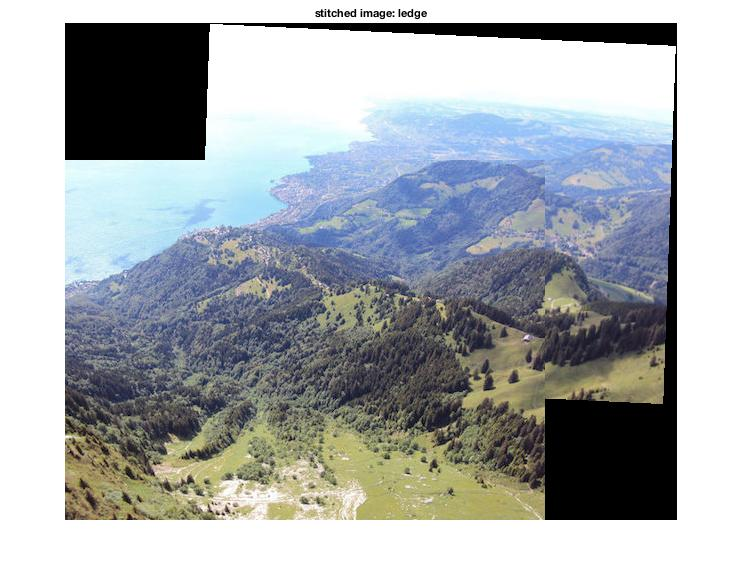
\includegraphics[width=1.2\textwidth]{ledge3.jpg}

Affine Transformation Matrix:
\vspace{10 mm}

Ledge.jpg

1.0049   ,   -0.0562   ,     143.6702;

0.0679   ,   0.9771    ,     -135.0352;

\end{center}

\newpage


Results for Pier.jpg
\begin{center}
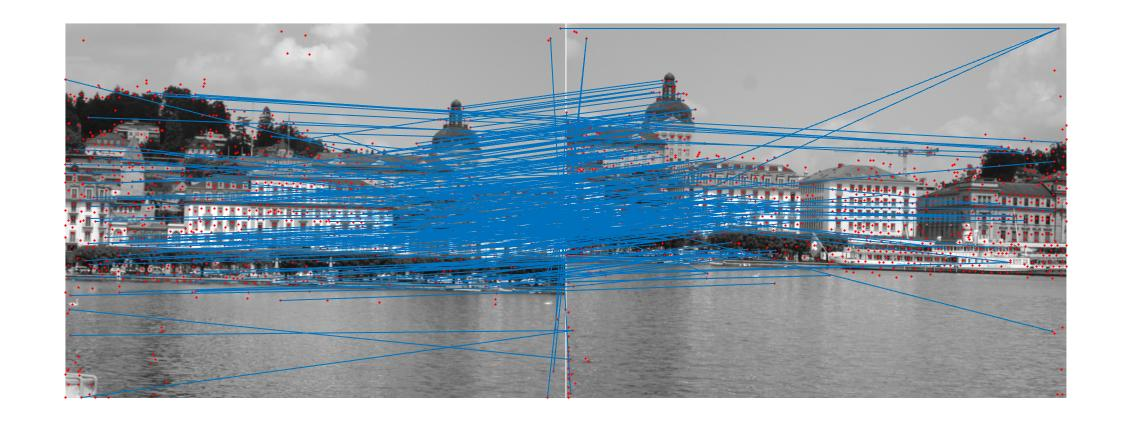
\includegraphics[width=1.2\textwidth]{pier1.jpg}

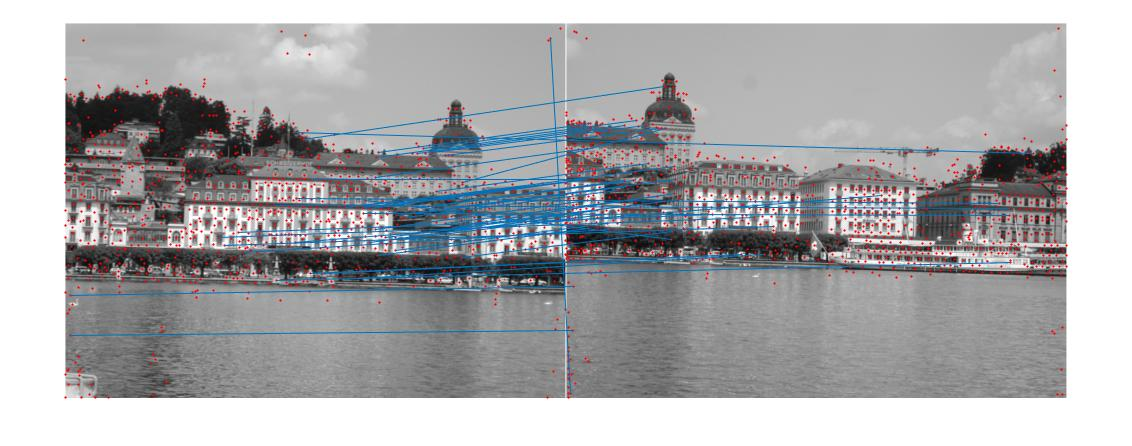
\includegraphics[width=1.2\textwidth]{pier2.jpg}
\newline
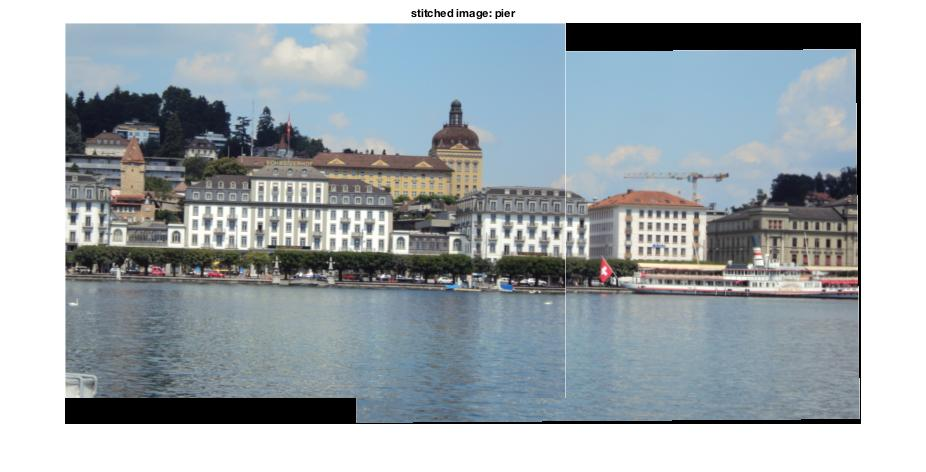
\includegraphics[width=1.2\textwidth]{pier3.jpg}

Affine Transformation Matrix:
\vspace{10 mm}

Pier.jpg

1.0078   ,   0.0108    ,    286.5016;

-0.0078  ,   0.9892    ,    29.4984

\end{center}

\newpage

Results for River.jpg
\begin{center}
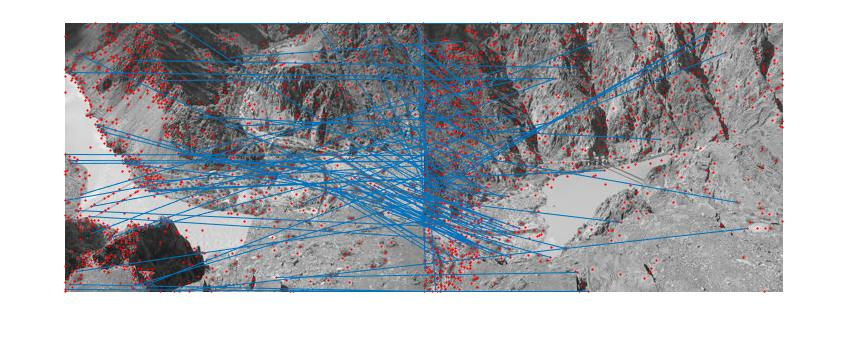
\includegraphics[width=1.2\textwidth]{river1.jpg}

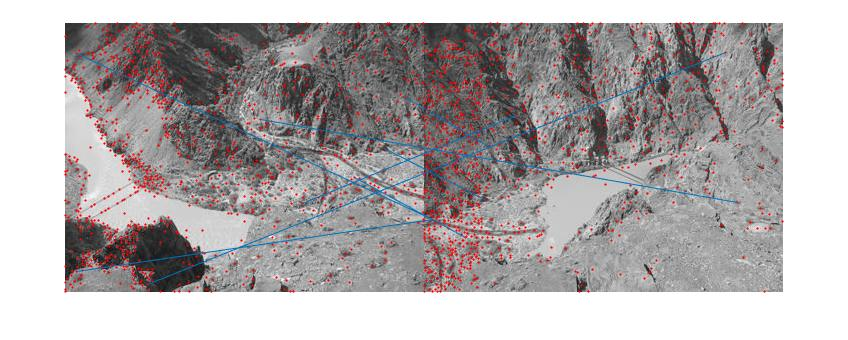
\includegraphics[width=1.2\textwidth]{river2.jpg}
\newline
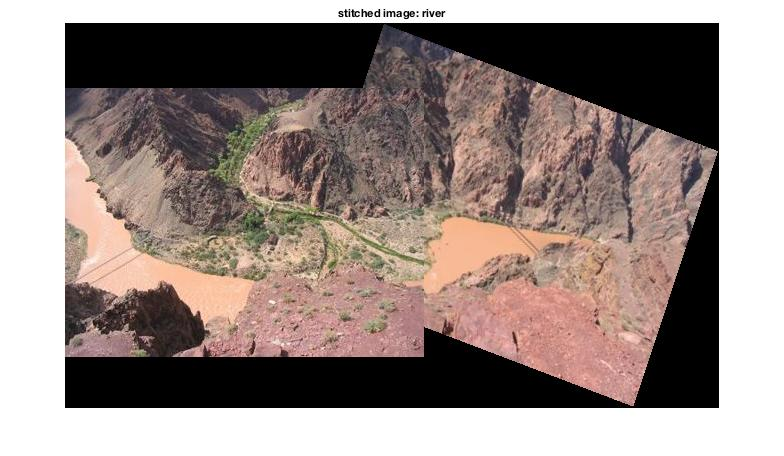
\includegraphics[width=1.2\textwidth]{river3.jpg}

Affine Transformation Matrix:
\vspace{10 mm}

River.jpg

0.9329   ,   -0.3276    ,    321.2789;

0.3539   ,   0.9487   ,  -63.7605;

\end{center}

\newpage

Results for Roof.jpg
\begin{center}
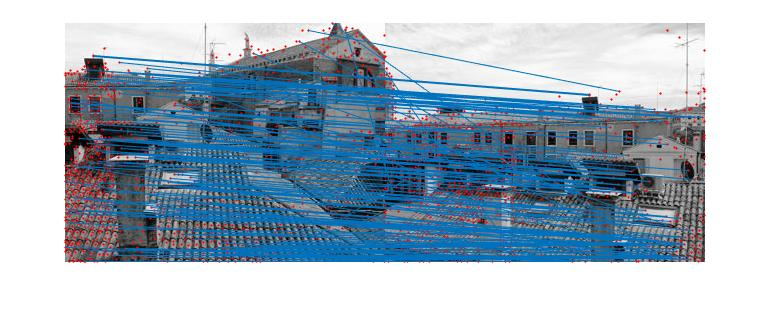
\includegraphics[width=1.2\textwidth]{roof1.jpg}

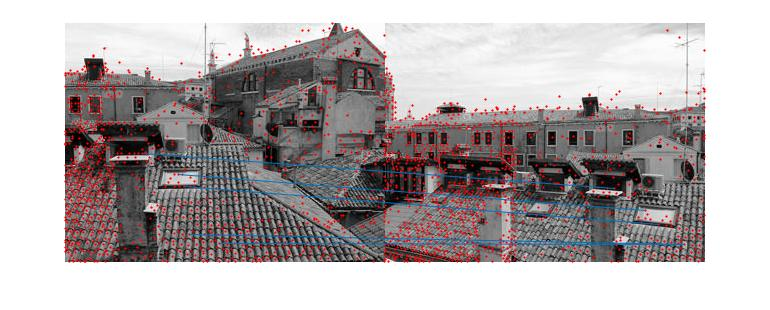
\includegraphics[width=1.2\textwidth]{roof2.jpg}
\newline
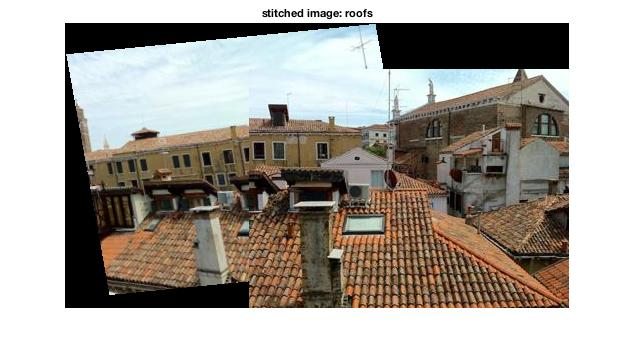
\includegraphics[width=1.2\textwidth]{roof3.jpg}

Affine Transformation Matrix:
\vspace{10 mm}

Roof.jpg

0.9693   ,   0.1818   ,  -183.3869;

-0.0951  ,   1.0119   ,  -15.1813;

\end{center}

\newpage

Results for Building.jpg
\begin{center}
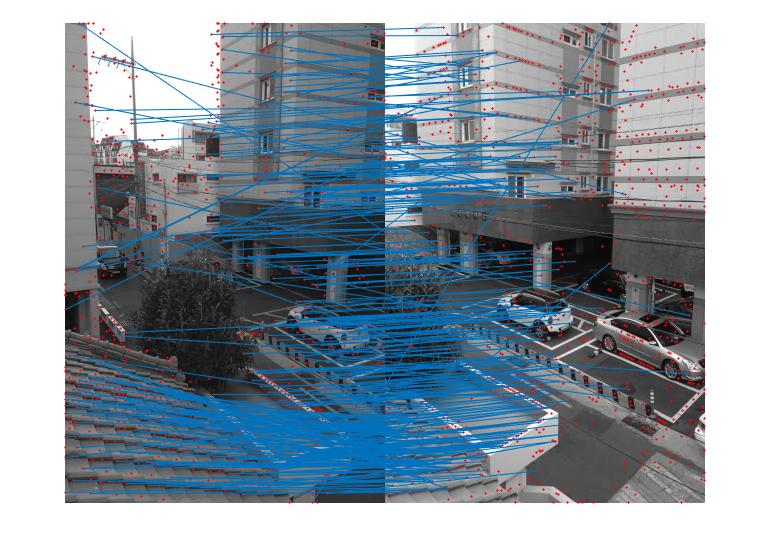
\includegraphics[width=1.2\textwidth]{building1.jpg}

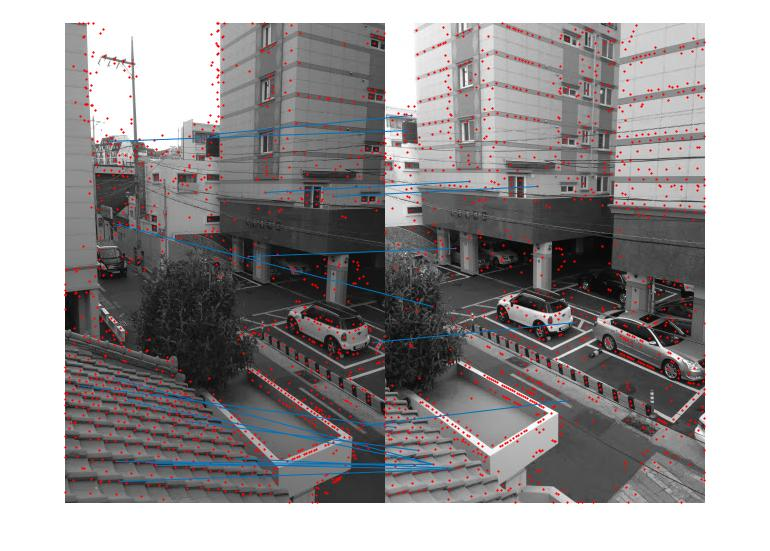
\includegraphics[width=1.2\textwidth]{building2.jpg}
\newline
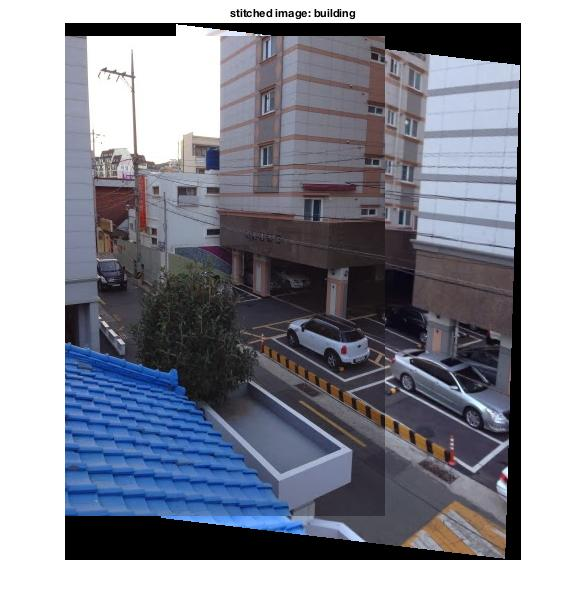
\includegraphics[width=1\textwidth]{building3.jpg}

Affine Transformation Matrix:
\vspace{10 mm}

Building.jpg

1.0775   ,   -0.0308    ,    110.6616;

0.1279   ,   1.0307     ,   -12.3888;

\end{center}

\newpage


Results for Uttower.jpg
\begin{center}
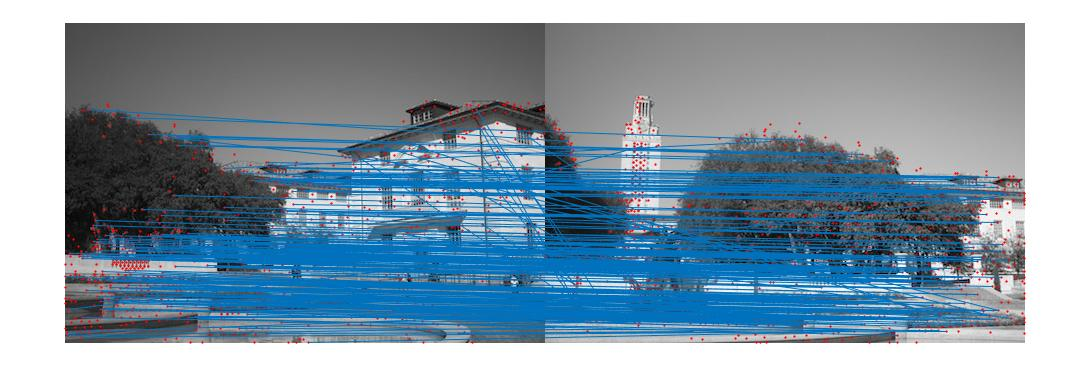
\includegraphics[width=1.2\textwidth]{uttower1.jpg}

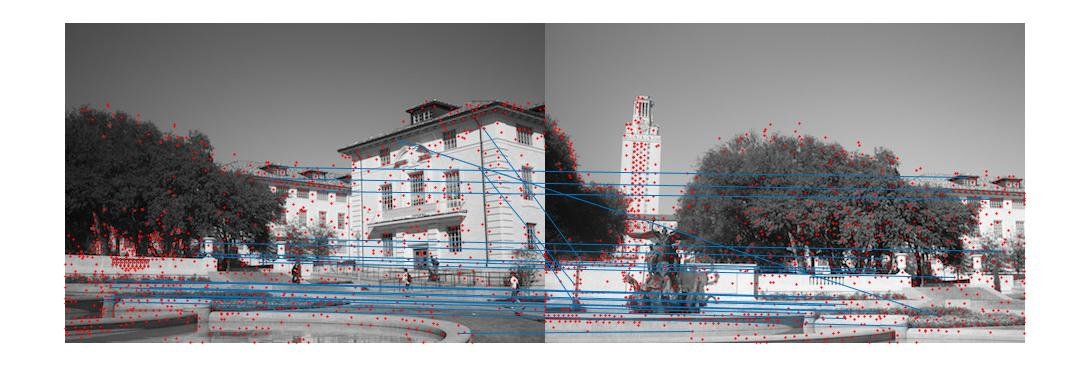
\includegraphics[width=1.2\textwidth]{uttower2.jpg}
\newline
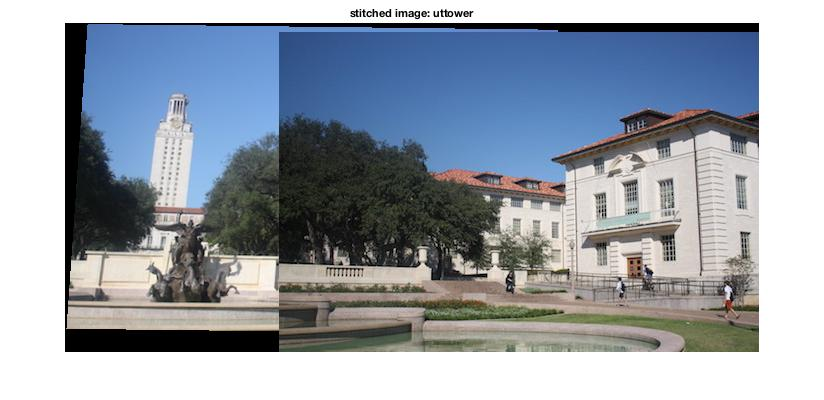
\includegraphics[width=1.2\textwidth]{uttower3.jpg}

Affine Transformation Matrix:
\vspace{10 mm}

Uttower.jpg

0.9806   ,   -0.0689    ,   -190.8962;

0.0202   ,   0.9570    ,    -11.9891;

\end{center}

\newpage

Code for \textbf{computeMatches.m}

\verbatiminput{computeMatches.m}


\newpage

Code for \textbf{ransac.m}

\verbatiminput{ransac.m}


\newpage
All Afine Transformation Matrices
\input{affine_transformation.txt}
\newpage

\end{document}
